\documentclass[twocolumn,showpacs,preprintnumbers,nofootinbib,prd,
superscriptaddress,10pt]{revtex4-1}

\usepackage{amsmath,amssymb}
\usepackage{amsfonts}
\usepackage[normalem]{ulem}
\usepackage{textcomp}
\usepackage{hyperref}
\usepackage{enumitem}
\usepackage{bm}
\usepackage{afterpage}
\usepackage{graphicx}
\graphicspath{{img/}} %setting img path
\usepackage{psfrag}
\usepackage{mathtools}
\usepackage{tensor}
\usepackage{layouts}
\usepackage{DejaVuSans}
\usepackage{epstopdf}
\usepackage[usenames,dvipsnames]{xcolor}
\usepackage[utf8]{inputenc}
\usepackage{multirow}
\usepackage{rotating}
\usepackage{tabularx}
\usepackage{ragged2e}
\usepackage{blindtext}
\usepackage{siunitx}
	\sisetup{output-decimal-marker={.}}
	
	%some math symbols
\newcommand{\R}{\mathbb{R}}
\newcommand{\N}{\mathbb{N}}
\DeclareMathOperator{\sign}{sign}
\renewcommand{\d}[1]{\ensuremath{\operatorname{d}\!{#1}}}
%argmin and argmax
\DeclareMathOperator*{\argmax}{arg\,max}
\DeclareMathOperator*{\argmin}{arg\,min}
\newcommand{\scalar}[2]{\langle #1|#2 \rangle}
\newcommand{\scalarnonorm}[2]{\langle #1|#2 \rangle_{\text{not normalized}}}
\newcommand{\rescalar}[2]{( #1 |#2 )}

% comments command
\newcommand{\stefano}[1]{{\textcolor{red}{\texttt{S: #1}} }}
\newcommand{\tim}[1]{{\textcolor{green}{\texttt{T: #1}} }}
\newcommand{\chinmay}[1]{{\textcolor{blue}{\texttt{C: #1}} }}
\newcommand{\oldnewtxt}[2]{\sout{#1}\textcolor{red}{#2}}

\begin{document}

	%%%%%%%%%%%%%%%%%%%%%%%%%%%%%%%%% ABSTRACT
\begin{abstract}

WRITEME

\end{abstract}
	
	%%%%%%%%%%%%%%%%%%%%%%%%%%%%%%%%% TITLE
	\title{mlgw NN}
	\author{Tim \surname{Grimbergen}}
        \affiliation{Institute for Gravitational and Subatomic Physics (GRASP),
		Utrecht University, Princetonplein 1, 3584 CC Utrecht, The Netherlands}
	%
	\author{Stefano \surname{Schmidt}}
		\email{s.schmidt@uu.nl}
        \affiliation{Institute for Gravitational and Subatomic Physics (GRASP),
		Utrecht University, Princetonplein 1, 3584 CC Utrecht, The Netherlands}
        \affiliation{Nikhef, Science Park 105, 1098 XG, Amsterdam, The Netherlands}
	%
	\author{Chinmay \surname{Kalaghatgi}}
        \affiliation{Institute for Gravitational and Subatomic Physics (GRASP),
		Utrecht University, Princetonplein 1, 3584 CC Utrecht, The Netherlands}
        \affiliation{Nikhef, Science Park 105, 1098 XG, Amsterdam, The Netherlands}
	%
	\author{Chris \surname{van den Broeck}}
        \affiliation{Institute for Gravitational and Subatomic Physics (GRASP),
		Utrecht University, Princetonplein 1, 3584 CC Utrecht, The Netherlands}
        \affiliation{Nikhef, Science Park 105, 1098 XG, Amsterdam, The Netherlands}
	\maketitle

	%%%%%%%%%%%%%%%%%%%%%%%%%%%%%%%%% BODY  
\section{Introduction}
\label{sec:intro}

\stefano{TODO:
\begin{itemize}
	\item Abstract
	\item Captions
	\item Citations
\end{itemize}
}

With almost a hundred of confirmed detections, Gravitational Waves (GW) astronomy is entering a mature state, where many loud GW events will force the scientific community to develop a fast analysis to deliver precision measurement. The recent transient catalogue GWTC-3 \cite{} is the latest achievment of the effort carried on by the LIGO-Virgo-KAGRA collaboration and it relies on both instrument and data analysis development.

A crucial element of the data analysis is the ability to generate accurate prediction of the GW signal emitted by a Binary Black Hole (BBH) system. Such waveforms are used for the expensive bayesian estimation of the parameters characterizing a BBH: the analysis of a single event requires the online generation of up to billions of waveforms.
As we move towards the next generation of detectors, it is mandatory to deploy accurate waveform models, that are fast and, at the same time, incorporate many physics effects. Failing to do this may lead to systematic errors in the parameter recovery, due to a bad modelling of the source.
This is challenging since, speed and accuracy are often at trade.

One important piece for a realistic BBH signal is the inclusion of the Higher Order Modes (HMs) of the multipole expansion of the waveform. For mass symmetric systems, the leading mode is orders of magnitude larger and including HMs doesn't affect the parameter estimation. On the other hand, it has been shown \cite{} that HMs are observable in very asymmetric binary systems, hence the need to include them to avoid any bias.

Throughout decades of developments, two families of models have been developed, both being able to incorporate HMs.
One family relies on the Effective One Body (EOB) formalism, which maps the complicated general relativistic binary system into a problem governed by an effective Hamiltonian. EOB models tend to be accurate but are quite costly to evaluate, since for each waveform one needs to solve the hamiltonian equation of motion.
On the other hand, the phenomenological waveforms are based on analytical expressions (within the post-newtonian formalism). They tend to be faster to evaluate, but don't achieve the same accuracy.
Both families, EOB and phenomenological, need to be calibrated with Numerical Relativity waveforms, computed by solving directly the Einstein equations. The calibration makes sure that a model retains its accuracy even close to merger, where an approximate treatment, such as the post-newtonian or EOB formalism are not applicable anymore.

Besides the standard families, surrogate waveform models have been developed for years with the intent of reproducing the output of a target model and of making feasible the usage of the underlying model. Several surrogates have been developed to accelerate several EOB models \cite{Gadre:2022sed}, even including HMs. While traditional surrogate models \cite{} build an empirical interpolant on the waveform space, a more modern approach relies on performing a regression using Machine Learning techniques \cite{}.

Among others, \cite{Schmidt:2020yuu} introduced a Machine Learning surrogate model, based on a dimensionality reduction scheme followed by a regression. In this work, we extend this model to HMs and we improve the accuracy of the regression. Our model marks a step towards the development of a fast, yet precise, waveform model by achieving state-of-the-art accuracy and speed, and will enable the accurate analysis of the next generation detectors' data.

We train our model on the widely used approximant \texttt{SEOBNRv4PHM} and we achieve a \tim{This is just the average mismatch then, right?} ??\% faithfulness when averaged across a wide range in the parameter space.
Our experiments showed that our model offers a substantial speed up with respect to the original model, matching the speed of the state-of-the-art surrogate models.

This paper is organized as follows. In Sec.~\ref{sec:model} we introduce the details of the model presented here, stressing the differences with the model in  \cite{Schmidt:2020yuu}.
Sec.~\ref{sec:performance} is devoted to the validation of our model: we will motivate our choice of several hyperparameters and perform an accuracy and speed study.
In Sec.~\ref{sec:end}, we present some final remarks and highlight future perspective.

%%%%%%%%%%%%%%%%%%%
\section{Building the model}
\label{sec:model}

A non-precessing BBH can be described by four {\it intrisic} parameters, which specify the two BH masses $m_1$ and $m_2$ and the z-component of the two spin $s_1$ and $s_2$.
Moreover, since the total mass $M = m_1 + m_2$ sets an overall amplitude scaling, a non-precessing BBH signal only depends on the mass ratio $q = m_1/m_2 \geq 1$ as well as on the spins. We may refer to these parameter as $\boldsymbol{\vartheta} = (q, s_1, s_2)$.
Besides the masses and spins, the gravitational wave emitted by the system depends also on luminosity distance to the source $d_L$, the inclination angle $\iota$ of the source and the reference phase $\varphi_0$: we call them {\it extrinsic}.

As it is standard, we expand the angular dependence on $\iota, \varphi_0$ of the {\it complex} waveform $h(t)$ in terms of a sum of spin -2 spherical harmonics.
A GW is then parameterized\footnote{Such parameterization is particularly convenient as it separates the waveform dependence over intrinsic and extrinsic parameters.} as~\cite{Estelles:2021gvs}:
\begin{align} \label{eq:h_parametrization}
	&h(t; d_L,\iota,\varphi_0, m_1, m_2, s_1, s_2) = h_+ + i h_\times \nonumber \\
		&\qquad= \frac{G}{c^2} \frac{M}{d_L}\sum_{\ell = 2}^{\infty} \sum_{m = -\ell}^{\ell} \tensor[^{-2}]{Y}{_{\ell m}}(\iota, \varphi_0) h_{\ell m}(t/M; \boldsymbol{\vartheta})
\end{align}
where we refer to the functions $h_{\ell m}(t; \boldsymbol{\vartheta})$ as {\it modes} of the waveform. We note that that, for non-precessing systems, $h_{\ell m} = (-1)^\ell h^*_{\ell -m}$, hence we will only consider modes with $m>0$.

The mode $(\ell, m) = (2,2)$ is by far the largest in amplitude, hence it is often referred to as the {\it dominant mode}. The other sub-dominant modes are few orders of magnitude smaller in amplitude and become more relevant (and measurable!) for high mass ratios \cite{}.

In this work, we introduce a Machine Learning model to perform a regression
\begin{align}\label{eq:objective}
	(q, s_1, s_2) &\longmapsto h_{\ell m}(t; \boldsymbol{\vartheta})
\end{align}
for each mode $(\ell,m)$.
The regression is designed to reproduce waveforms from a given dataset; such waveforms can be generated by {\it any} time-domain approximant.

We decompose each mode in amplitude and phase
\begin{equation}
	h_{\ell m}(t; \boldsymbol{\vartheta}) = A_{\ell m}(t; \boldsymbol{\vartheta}) e^{i \phi_{\ell m}(t; \boldsymbol{\vartheta})}
\end{equation}
and, for each mode, we perform a regression for amplitude and phase separately. The regression scheme closely follows \cite{Schmidt:2020yuu} and relies on:
\begin{enumerate}[label=(\alph*)]
	\item a suitable vector representation of the regression target by choosing a fixed time grid
	\item a Principal Component Analysis (PCA) model to reduce the dimensionality of each waveform
	\item an Artificial Neural Network (ANN) regression to learn the dependence on $\boldsymbol{\vartheta}$ of the reduced waveform
\end{enumerate}

While the first two elements are unchanged from the previous work, the ANN regression is first introduced here. Indeed a NN has more representation power than the Mixture of Experts (MoE) model \cite{Jacobs1991AdaptiveMoE}, used in \cite{Schmidt:2020yuu}: the change was needed to achieve better accuracy for the model.

\subsection{Dataset creation}
\label{sec:dataset}

To construct a dataset, we follow \cite{Schmidt:2020yuu} and we set a dimensionless time grid. We construct the grid by setting $D$ points equally spaced in $\tau^\alpha$, where $\tau$ is the physical time scaled by the total mass of the system $M$: $\tau = t/M$. Using the findings of \cite{Schmidt:2020yuu}, we set $D = \text{2000}$ and $\alpha = \text{0.5}$.
%
This is a good compromise between the need of having a faithful representation of the waveform (which requires a large grid) and the need of having a compact model (which points to a sparse grid).

The starting point of the grid $\tau_0$ sets the length of the waveform that our model is able to generate. We choose $\tau_0 = \SI{2}{s/M_\odot}$ and we populate the dataset with $68000$ waveforms.

To make sure that the distribution of $q$ is skewed towards towards the boundaries, where the regression is less accurate, we sample the mass ratio $q$ in the range $[1,10]$ with the following procedure:
\begin{itemize}
	\item We sample $q_1, \hdots, q_5 \sim \mathcal{U}_{[1,10]}$
	\item We sample $x \sim \mathcal{U}_{[0,1]}$
	\item We select q, based on the value of $x$:
	\begin{itemize}
		\item If $x \in [0,0.3)$, $\min q_1, \hdots, q_5$
		\item If $x \in [0.3, 0.8)$, $q_1$
		\item If $x \in [0.8, 1]$, $\max q_1, \hdots, q_5$
	\end{itemize}
\end{itemize}
where $\mathcal{U}_{[a,b]}$ is the uniform distribution in $[a,b]$.
The spins are drawn uniformly in the range $[-0.99, 0.99]$.
\stefano{This mechanism is complicated but it's late to change it}

Once a time grid is set, we evaluate all the modes (amplitude and phase) on the time grid and represent them as vectors in $\R^D$.
We then create a dataset $\{X, Y\}$ of $N$ elements. Each row of the dataset is of the form:
\begin{align}
	X &= [q, s_1, s_2] \\
	Y &= [\boldsymbol{A}^T_{\ell m}, \boldsymbol{\phi}^T_{\ell m}, \hdots ] 
\end{align}
%
The dataset $Y$ gathers the amplitude and phase for the different modes in the dataset.
We include all the modes available in \texttt{SEOBNRv4PHM}: $(\ell, m) = \{(2,2),(2,1), (3,3), (4,4), (5,5)\}$.

In what follows we will refer to any of the vectors $\boldsymbol{A}_{\ell m}$ or $\boldsymbol{\phi}_{\ell m}$ as $\boldsymbol{f}$.
Note that we use the same grid for all the modes.

\subsection{Dimensionality reduction}
\label{sec:PCA}

It is unfeasibile to perform a regression targeting a large dimensional vector such as $\boldsymbol{f} \in \R^D$. For this reason, in \cite{Schmidt:2020yuu} we introduced a Principal Component Analysis (PCA) dimensionality reduction scheme.
It is an approximately invertible linear mapping between a vector $\boldsymbol{f} \in \R^D$ in a large dimensional space to lower dimensional vector  $\boldsymbol{g} \in \R^K$: \tim{I put a hat on the $\mathbf{f}$ in equation 7 since otherwise it looks like the operations is actually mathematically invertible}
%
\begin{align}
	\mathbf{g} = H (\mathbf{f} - \boldsymbol{\mu}) \label{eq:PCA_reduction_model}\\
	\hat{\mathbf{f}} = H^T \mathbf{g} + \boldsymbol{\mu} \label{eq:PCA_reconstruction_model}
\end{align}
where $\boldsymbol{\mu} \in \R^D$ and $H$ is a $K \times D$ matrix. The rows $H_{i:}$ of $H$, also called {\it Principal Components} (PC), form an orthonormal set of vector, i.e. it holds ${\sum_{k=1}^D H_{ik} H_{kj} = \delta_{ij}}$.
The PCs are the first $K$ eigenvectors of the $D \times D$ covariance matrix of the dataset, as described in \cite[Sec. 12]{murphy2012machine}.

One can have a deeper insight on PCA considering the following formula for the reconstructed vector $\mathbf{f}$ (setting $\boldsymbol{\mu}=0$ without loss of generality):
\begin{equation} \label{eq:perturbative_exp}
	\mathbf{f} = \sum_{i=1}^K \langle \mathbf{f} | H_{i:} \rangle \; H_{i:}
\end{equation}
%
where $\langle \cdot | \cdot \rangle$ is the usual scalar product.

Since less important PCs are more orthogonal to data, the typical magnitude of $g_i = \langle \mathbf{f} | H_{i:} \rangle$ decreases as $i$ increases.\footnote{For this reason PCA can be seen as a perturbative expansion on the basis vectors $H_{i:}$, where the accuracy is roughly measured by the eigenvalues of the first neglected PC. Increasing the number K of PCs considered increases the accuracy of the model (but also the complexity of the model).}.
As a consequence, the regression for a lower order PC needs to be more accurate than the one for the higher order PC. This will be taken care by a suitable choice for the loss function for the regression (see next section).

%%%%%%%%%%%%%%%%%%%%%%%%%%%%%%%%%%%%%%%%%%%%%%%%%%%%%%%%%%%%%
\begin{figure*}[t]
	\begin{multicols}
		\centering
		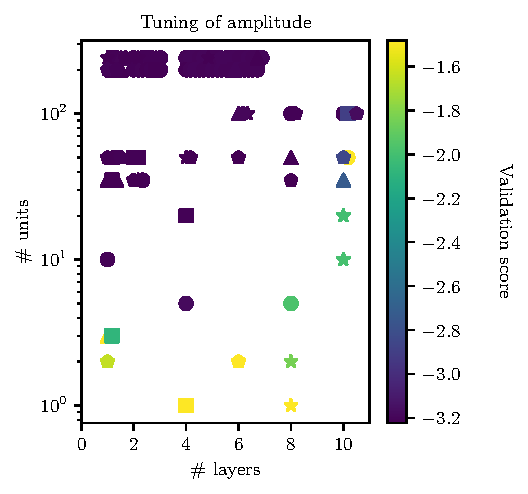
\includegraphics[scale = 0.9]{tuning_amp}\hfill
		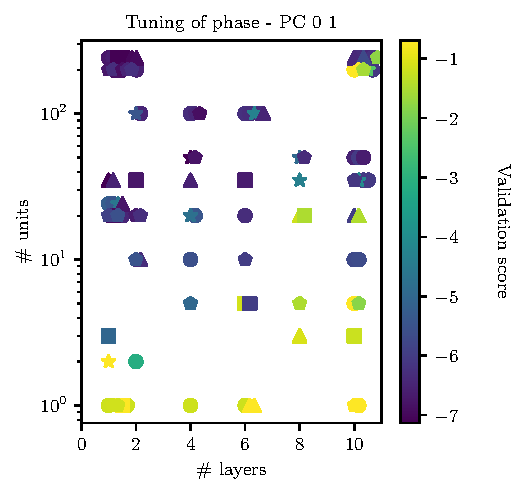
\includegraphics[scale = 0.9]{tuning_ph_01}
	\end{end}
	\begin{multicols}
		\centering
		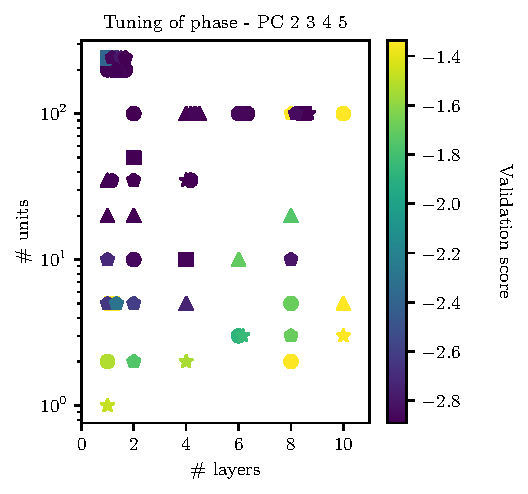
\includegraphics[scale = 0.9]{tuning_ph_2345}\hfill
		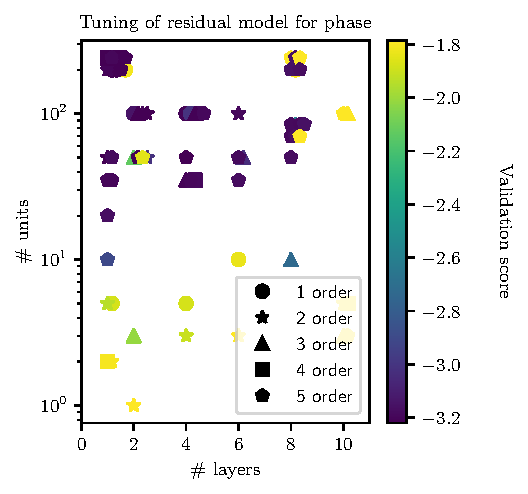
\includegraphics[scale = 0.9]{tuning_ph_01_residual}
	\end{end}
	\caption{}
	\label{fig:tuning}
\end{figure*}
%%%%%%%%%%%%%%%%%%%%%%%%%%%%%%%%%%%%%%%%%%%%%%%%%%%%%%%%%%%%%

\subsection{Neural network regression}
\label{sec:NN}

An Artificial Neural Network (ANN) is a popular regression model, consisting of a powerful parametric function, whose parameters (or weights), when properly set, can represent a large variety of relations between input and output.
An ANN is built by stacking together $N_\text{L}$ layers in such a way that the output of a layer is the input of the following layer. \tim{$D$ is already a reserved variable for the number of grid points, so I put some more primes on the $D's$ in this section to avoid confusion.} Each layer is a function $L: \R^D\prime \rightarrow \R^{D^\prime\prime} $ and has the following functional form

\begin{equation}
	\boldsymbol{y} = a(W^{\prime}_{\prime\prime}\boldsymbol{x})
\end{equation}
%
Where $W^{\prime}_{\prime\prime}$ is a $D^\prime\prime \times D\prime$ matrix and $a: \R \rightarrow \R$ is an activation function that acts elementwise on the vector $W^{\prime}_{\prime\prime}\boldsymbol{x}$.
Each component $y_i$ of the output of the layer is called a node and the number of nodes is a tunable parameter, controlling the representative power of the layer.

An ANN $\mathcal{N}$ is obtained by composing $N_\text{L}$ different layers (each with a suitable number of nodes):
%
\begin{equation}
	\mathcal{N}_W = L_{N_\text{L}} \circ \hdots \circ L_2 \circ L_1
\end{equation}
%
where we denote by $W$ the set of all the parameters the ANN depends on.

The number of layers, together with the number of nodes per layer are hyperparameters that need to be carefully chosen, to balance model accuracy and model complexity.
Another important choice is the activation function: several possible choices are possible, the most popular being the {\it sigmoid}, the hyperbolic tangent or the so called ReLU function. In our work, we consider the sigmoid function between all layers, except for the very last layer which has linear/identity activation so that negative values are also possible.

Once the ANN is set up, we need to set its weights to the values that achieve our regression task.
This procedure is called training, where we minimize a loss function with respect to the weights $\boldsymbol{W}$ of the model.
The loss function depends on the dataset at hand ${\{\boldsymbol{x}_i, \boldsymbol{y}_i\}_i}$.
Mathematically, the weights are given by:
%
\begin{equation}\label{eq:loss_general}
	\boldsymbol{W} = \argmin_W \mathcal{L}(W; \{\boldsymbol{x}_i, \boldsymbol{y}_i\}_i)
\end{equation}

The minimization of the loss function is performed by stochastic gradient descent (SGD) \tim{More specific: the optimizer is the "Nadam" optimizer https://keras.io/api/optimizers/Nadam/}, which relies on the gradients $\partial_W \mathcal{L}$ of the loss function. The gradients are computing through the backpropagation algorithm \cite{}.

To perform our regression $\theta \longmapsto \boldsymbol{g}$, we employ an ensemble of networks that suitably combined delivers accurate results.
To improve the representative power or the ANN, we employ feature augmentation on the vector $\boldsymbol{\vartheta} = (q, s_1, s_2)$, effectively using the augmented vector $\tilde{\boldsymbol{\vartheta}}$ as input for the regression. Although different ANN's will need different features, we will for convenience abuse the notation $\tilde{\boldsymbol{\vartheta}}$ to any augmented vector. Indeed, the features to add need to be chosen with a validation process: this will be discussed in the next section.

Before the training, the regression targets $\boldsymbol{y}_i$ are scaled such that $\boldsymbol{y}_i \rightarrow \frac{\boldsymbol{y}_i}{\boldsymbol{w}}$, where $\boldsymbol{w}$ keeps the maximum of $|\boldsymbol{y}_i|$ along each axis. %${w}_j = \max_i(|(\boldsymbol{y}_i)_j|)$.
In this way all the regression targets span the same order or magnitude, making the regression task easier.

For the amplitude $\boldsymbol{A}_{\ell m}$ of each mode, we employ a single ANN $\mathcal{N}_{A_{\ell m}}$ that predicts the first four PCA components.
The predicted amplitude $\hat{\boldsymbol{A}}_{\ell m}$, including the PCA reconstruction, has the following form:
\begin{equation}\label{eq:amp_pred}
	\hat{\boldsymbol{A}}_{\ell m}(\boldsymbol{\vartheta}) = \boldsymbol{\mu}_{A_{\ell m}} + H_{A_{\ell m}}^T \mathcal{N}_{A_{\ell m}}(\tilde{\boldsymbol{\vartheta}})
\end{equation}

For the phase $\boldsymbol{\phi}_{\ell m}$, we employ one ANN $\mathcal{N}_{\phi_{\ell m}\text{- 12}}$ to predict only the first two PCA components.
Another ANN will take care of the remaining components $\mathcal{N}_{\phi_{\ell m}\text{- 2345}}$ \tim{Should we refer to \cite{Schmidt:2020yuu} to argue why only these PCA components have to be considered?}.
On top of this, we build an additional ANN $\mathcal{N}_{\phi_{\ell m}\text{- residual}}$ to target the residual of the predictions of $\mathcal{N}_{\phi_{\ell m}\text{- 12}}$ \tim{Is the term "residual" a well-known term (or clear enough from context) or does it require more explanation?}.
The scheme make sure that the first two PCs are predicted with much larger accuracy than the others. Indeed, the reconstructed WF depends largely on the first two components and a small fractional error can potentially have a large impact on the overall accuracy.

The predicted phase $\hat{\boldsymbol{\phi}}_{\ell m}$ is then given by:
%
\begin{equation}\label{eq:ph_pred}
	\hat{\boldsymbol{\phi}}_{\ell m}(\boldsymbol{\vartheta}) = \boldsymbol{\mu}_{\phi_{\ell m}} + H_{\phi_{\ell m}}^T 
	\begin{pmatrix}
        \mathcal{N}_{\phi_{\ell m}\text{- 12}}(\tilde{\boldsymbol{\vartheta}}) + \mathcal{N}_{\phi_{\ell m}\text{- residual}}(\tilde{\boldsymbol{\vartheta}}) \\
        \mathcal{N}_{\phi_{\ell m}\text{- 2345}}(\tilde{\boldsymbol{\vartheta}}) \hfill
	 \end{pmatrix}.
\end{equation}


We train our model using the PCA dataset, obtained by PCA reducing the training set. Each ANN is trained using the following loss function: \tim{I know in the definition of the custom loss function the w for the weights is inside the square, but (at least in the fitNN function that I wrote) I think we take the square root of $\boldsymbol{w}$ as input of the loss weights, so that the $\boldsymbol{w}$ in the definition below should be outside of the square...}
\begin{equation}\label{eq:loss}
	\mathcal{L} = \frac{1}{N} \sum_{i=1}^N \Bigl((\mathcal{N}(\boldsymbol{\vartheta}_i) - \boldsymbol{y}_i)}\boldsymbol{w} \Bigr)^2
\end{equation}
%
where $\boldsymbol{y}_i$ is the (scaled) regression target of each network and $\boldsymbol{w} \in \R^K$ takes into account the fact that different PCs have different orders of magnitude.

The network is implemented and trained using the python package \texttt{keras} \cite{chollet2015keras}, built on \texttt{tensorflow} backend \cite{tensorflow2015-whitepaper}.

%%%%%%%%%%%%%%%%%%%
\section{Performance study}
\label{sec:performance}
In this section, we first study how the model performance depends on the different choices of hyperparameters (network architecture, learning rate, features etc...).
The architecture details of the model (chosen after hyperparameters tuning) are reported in Tab.~\ref{tab:model}.
We then evaluate the faithfulness of our model and report the speed up that we obtain when using \texttt{mlgw-NN} instead of the training model \texttt{SEOBNRv4PHM}.

To measure the discrepancy between two waveforms  $h_1$, $h_2$, we define a scalar product:
\begin{equation}
	\rescalar{h_1}{h_2} = 4 \Re \int_{-\infty}^{\infty} \text{d}f \; \frac{{\tilde{h}^*}_1(f) \tilde{h}_2(f)}{S_n(f)}
\end{equation}
where $\tilde{\phantom{h}}$ denotes the Fourier transform and $S_n(f)$ is the Power Spectral Density (PSD) of the detector's noise.
We can use the scalar product to normalize a waveform: we denote by $\hat{h} = \frac{h}{\sqrt{\rescalar{h}{h}}}$ the normalized waveform $h$.

To measure the discrepancy between two individual modes $h^1_{\ell m}$ and $h^2_{\ell m}$, we define the {\it match} $\mathcal{M}$:
\begin{equation}\label{eq:match}
	\mathcal{M} = \max_t \; \rescalar{\hat{h}^1_{\ell m}}{\hat{h}^2_{\ell m} e^{i 2\pi ft}}
\end{equation}
where $h e^{i 2\pi ft}$ denotes (with a slight abuse of notation) $h$ translated in time by a factor of $t$.
We call {\it mismatch} the quantity $\mathcal{F} = 1 - \mathcal{M}$.

The match defined above amounts to the the search statistics being used for matched filtering searches of non-precessing/non-HM signals \cite{}.
A different stastics is needed to search for HM signals, hence the match defined above is not suitable to compare two different waveforms with HM content Eq.~\eqref{eq:h_parametrization}.
In this case, we need to compare the two polarizations $h_+$, $h_\times$ of a waveform with a signal $s$ observed at the detector:
\begin{equation}
	s = F_+ h_+ + F_\times h_\times
\end{equation}
where $F_+, F_\times$ are called antenna pattern functions, depending on the sky location of the source and on the polarization angle \cite{}.

We are then ready to introduce the {\it symphony match}\footnote{The name comes from the paper \cite{} first introducing it} between a signal $s$ and a waveform $h$:
\begin{equation}\label{eq:match_sym}
	\mathcal{M}_\mathrm{sym} = \max_t \;
		\frac{ \rescalar{\hat{s}}{\hat{h}_+}^2 + \rescalar{\hat{s}}{\hat{h}_\times}^2 - 2 \rescalar{\hat{h}_\times}{\hat{h}_+} \rescalar{\hat{s}}{\hat{h}_+} \rescalar{\hat{s}}{\hat{h}_\times}}
		{1-\rescalar{\hat{h}_\times}{\hat{h}_+}^2}
\end{equation}
note that the $\mathcal{M}_\mathrm{sym}$ depends on the signal $s$, hence it depends on the sky location and polarization angle.
As above, we define the symphony mismatch as $\mathcal{F}_\mathrm{sym} = 1 - \mathcal{M}_\mathrm{sym}$.
\stefano{I didn't want to go into too many details here but maybe the whole discussion is unclear and needs more details}

\subsection{Hyperparameters tuning}
\label{sec:hyperparameter}

\begin{table}[t]
	\begin{tabular}{ l|c|c|c|c } 
		Network & \texttt{n-layers} & \texttt{units} & \texttt{features} & \texttt{order} \\
		\hline\hline
			$\mathcal{N}_{A_{\ell m}$
				& 1 & 35 & $\mathcal{M}_c, \chi_\text{eff}$ & 1 \\
			$\mathcal{N}_{\phi_{\ell m}\text{- 12}}$ 
				& 2 & 50 & $\mathcal{M}_c, \eta, \log q, \chi_\text{eff}$ & 3 \\
			$\mathcal{N}_{\phi_{\ell m}\text{- 2345}}$
				& 1 & 50 & $\mathcal{M}_c, \eta, \log q, \chi_\text{eff}$ & 1 \\
			$\mathcal{N}_{\phi_{\ell m}\text{- residual}}$
				& 5 & 50 & $\mathcal{M}_c, \eta, \log q, \chi_\text{eff}$ & 2 \\
	\end{tabular}
	\label{tab:model}
	\caption{Architecture of the 4 ANNs employed to generate each mode. For each ANN we report the number of layers and the number of units per layer. We perform data augmentation by adding all the polynomials terms in the chosen features.
	The architecture have been chosen after hyperparameter tuning (see Fig.~\ref{fig:tuning}).
	Among the features, we use the chirp mass $\mathcal{M}_c =\frac{(m_1 m_2)^{3/5}}{(m_1+m_2)^{1/5}}$, the symmetric mass ratio $\eta = \frac{m_1 m_2}{(m_1+m_2)^2}$ and the effective spin parameter $\chi_\text{eff} = \frac{m_1 s_\text{1z} +m_2 s_\text{2z}}{m_1+m_2}$.
	}
\end{table}

\begin{figure}[t]
	\centering
	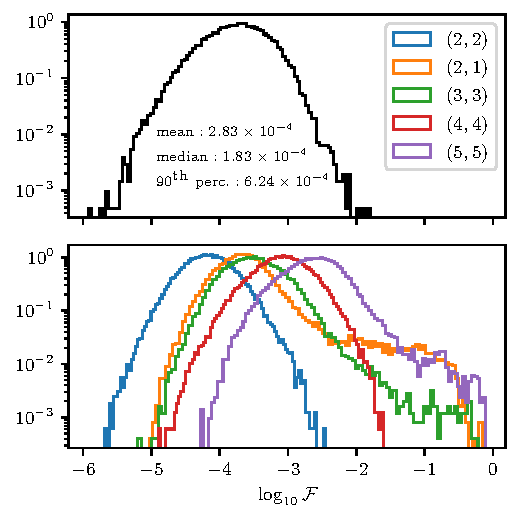
\includegraphics[scale = 1]{accuracy}
	\caption{}
	\label{fig:accuracy_hist}
\end{figure}

\begin{figure*}[t]
	\centering
	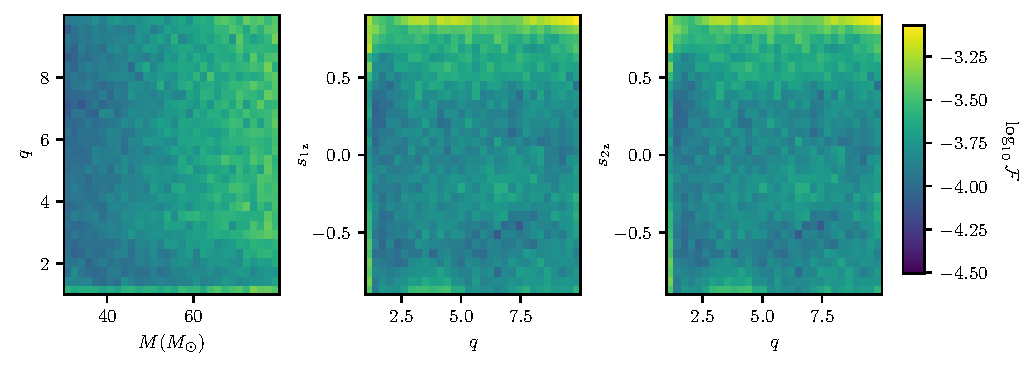
\includegraphics[width=\textwidth]{colormesh}
	\caption{WRITEME}
	\label{fig:countour_plots}
\end{figure*}

\begin{figure*}[t]
	\centering
	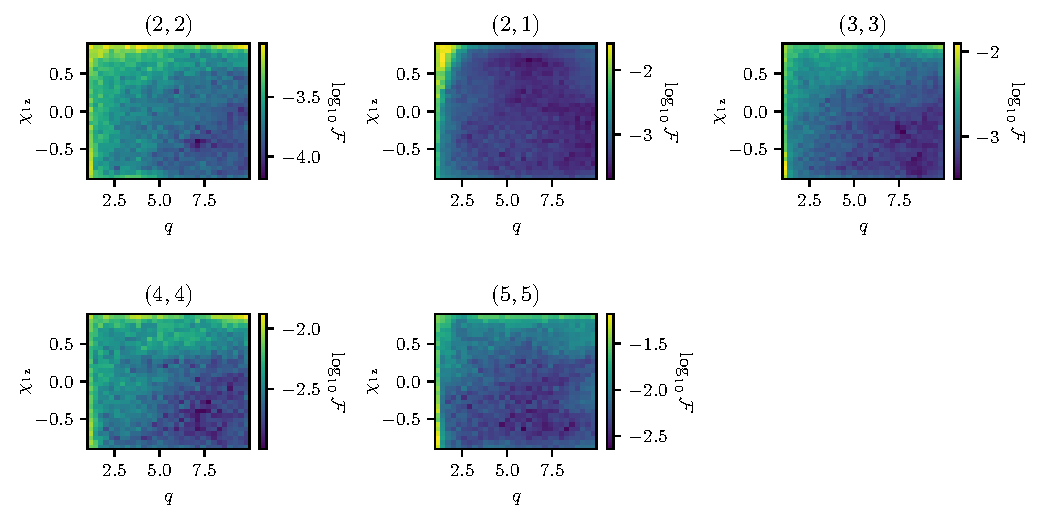
\includegraphics[width=\textwidth]{colormesh_modes}
	\caption{WRITEME}
	\label{fig:countour_plots_modes}
\end{figure*}

The performance of the model depends on a number of crucial choices about some non-trainable parameters, usually called hyperparameters. The hyperparameters usually defines the architecture of the ANN as well as some parameters relevant to the training.
Setting the right values for the hyperparameters is crucial for the ANN performance, as one needs to balance between accuracy and speed: this procedure is called {\it hyperparameters tuning} and can be done authomatically to optimize manual work and to make sure to find a good minimum.

We optimize the following hyperparameters:
\begin{multicols}{2}
	\begin{itemize}
		\item \texttt{n-layers}: number of layers in the ANN
		\item \texttt{units}: number of hidden features per layer
		\item \texttt{features}: features to use for data augmentation
		\item \texttt{order}: the data will be agumented with all the monomials of the chosen features up th given order
	\end{itemize}
\end{multicols}

For each of the 4 ANN useful to reproduce a single mode (see Eq.~(\ref{eq:amp_pred}-\ref{eq:ph_pred})), we train a network for different combinations of hyperparameters. The figure of merit of each hyperparameter choice is the logarithm of the loss function Eq.~\eqref{eq:loss} evaluated on the validation set. \stefano{@Tim: is this true?}
For our experiments we only use the dataset of the $(2,2)$ mode and we employ the package \texttt{keras-tuner} \cite{omalley2019kerastuner}.

We report our results in Fig.~\ref{fig:tuning}, where each combination of hyperparameters tested is represented in the \texttt{n-layers}-\texttt{units} plane and coloured by the validation scored. 
We can see that all the four ANN share the same trend: the most effective way to improve regression accuracy is to increase the number of units as opposed to the number of layers.
The number of layers is far more important the extra features added and the polynomial order for data augmentation.

Furthermore, we note that the regressions for the amplitude and for the high phase PCs (i.e. compoenents 2,3,4,5) can be performed with a smaller model, compared to the models for the first two PCs of the phase. This can be explained by the fact that most of the physical information is stored in the first two components of the phase, making this an harder regression problem.

In table Tab.~\ref{tab:model} we report the final hyperparameter choice we made for each of the networks. The architectures are the same across the different modes considered.

As discussed above, we note that models $\mathcal{N}_{A_{\ell m}$ and $\mathcal{N}_{\phi_{\ell m}\text{- 2345}}$ are very simple, having only one layer and a small polynomial order, while the other ANNs have a more complicated architeture.
We note here that an accurate ANN for the residuals of the phase is crucial to obtain a good accuracy: indeed $\mathcal{N}_{\phi_{\ell m}\text{- residual}}$ is the most complex model we employ, meaning that the residual phase dataset is the ``hardest" to learn.

\subsection{Accuracy study}\label{sec:accuracy}

To test the accuracy of our model, we generate a test set with $50000$ randomly chosen waveforms generated with the training model \texttt{SEOBNRv4PHM}.
The waveforms masses are characterized by a total mass in the range $[30, 80] M_\odot$, by a mass ratio $q \in [1, 10]$. The spins are chosen in the range $[-0.99, 0.99]$ and the inclination angle $\iota$ and reference phase $\varphi_0$ are drawn uniformly from a sphere.
We set the starting frequency in the range $[10, 20]Hz$.

In Fig.~\ref{fig:accuracy_hist}, we report the histogram of the distribution of the mismatches between \texttt{mlgw} and the test waveforms. The upper part refers to the mismatches Eq.~\eqref{eq:match_sym} computed on the overall waveforms (with sky location sampled uniformly over the sky); the lower box refers to mismatches computed mode by mode with Eq.~\eqref{eq:match}.

First of all, we note that the model show very high faithfulness. With a median value of $2\times 10^{-4}$ and with virtually no signals with a ``symphony" mismatch higher than $10^{-2}$, \texttt{mlgw} is indistinguishable from \texttt{SEOBNRv4PHM} for the current generation detectors \cite{WF_systematics}.
The faithfulness for the $(2,2)$ mode is even higher with no signals with mismatch higher than $2\times 10^{-3}$.
On the other hand, the higher order modes are less accurately reproduced than the dominant mode. In particular, for the modes $(2,1), (3,3), (5,5)$ a limited number of waveforms show very high mismatches $\mathcal{O}(1)$.

The cause of the decreased faithfulness for sub-dominant modes needs more investigation. However, it likely due to the fact that the physics of subdominant modes is less understood, hence the uncertainties in waveform modelling results in a more noisy regression for the ANN to learn.
This problem can be probably mitigated by using a larger network for such modes. Indeed, we tuned the hyperparameters on the $(2,2)$ (an ``easy" regression target): performing a tuning on the dataset of such modes might reveal that our chosen architecture is not optimal.

In Fig.~\ref{fig:countour_plots} we report the dependence of the ``symphony" mismatch as a function of the different orbital parameters.
From the figure, it is manifest that the model has very stable performance across the parameter space.
The faithfulness decreases for high positive values of the spins and for mass ratio $q\sim 1$: such cases are at the boundaries of the waveform dataset, hence they correspond to extreme values in the PCA reduction, making harder for the network to predict such cases. Despite this, in such ``extreme" regions, the average mismatch is still of the order of $10^{-4}$.
We also note that for $q\sim 1$, the sub-dominant modes have a vanishing amplitude: a large mismatch in the sub-dominant mode for $q\sim 1$ has very little impact on the overall waveform Eq~\eqref{eq:h_parametrization}.

In Fig.\ref{fig:countour_plots_modes}, for each mode we report the mismatch as a function of the mass ratio and of $s_\text{1z}$. One more time, we can see that the model faithfulness decreases for low mass ratios and for high spins. Moreover, the subdominant modes shows a poorer performance as compared to the dominant one.

\subsection{Timing study}
\label{sec:timing}

A speed up in the waveform generation is the main motivation to build a ML waveform generator; for this reason it is crucial to assess the gain in waveform generation time.
For this reason, we use our test set to measure the ratio between the time to generate a waveform with \texttt{SEOBNRv4PHM} and \texttt{mlgw}. Our model offers further speed by generating waveform in batches: in this case, some operations are efficiently parallelized and happen more efficiently.
We report our findings in Fig.~\ref{fig:timing_hist}.

We achieve a speed up between a factor of $100$ and $200$, depending on the length of the waveform. For waveform batch generation, the speed up can be twice as much, ranging between $200$ and $400$.
The speed up achieved by \texttt{mlgw} is slightly larger than the one obtained by a surrogate model \texttt{SEOBNRv4PHMSur} obtained with standard techniques \cite{Gadre:2022sed}.

\begin{figure}[t]
	\centering
	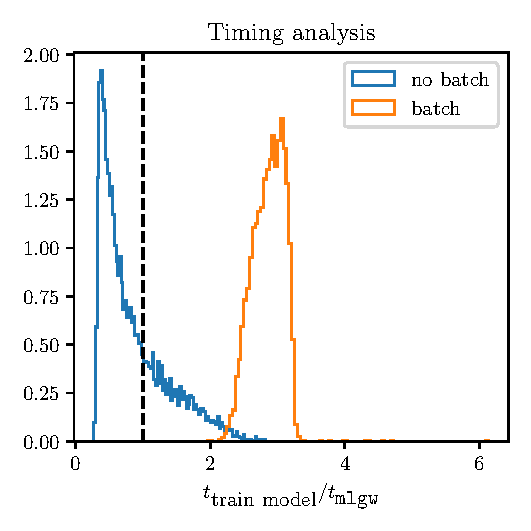
\includegraphics[scale = 1]{timing}
	\caption{}
	\label{fig:timing_hist}
\end{figure}

%%%%%%%%%%%%%%%%%%%

\section{Final remarks and future prospects}
\label{sec:end}

Building over our previous work \cite{}, we generate a ML surrogate model \texttt{mlgw} able to reproduce with very high fidelity the output of the widely used approximant \texttt{SEOBNRv4PHM}. \texttt{mlgw} can generate wavforms in a rectangle $q\times s_\text{1z} \times s_\text{2z} = [1,10]\times[-0.9,0.9]\times[-0.9,0.9]$ with on (reduce) grid of maximum length of $\SI{2}{s/M_\odot}$.
Our model offers a two orders of magnitude speed up over the training model, without trading for accuracy, hence it is an attractive alternative for any data analysis application.
Our method is fully general and is applicable to any chirp-like gravitational wave signal.
To encourage new applications, we release our code (and our trained model) publicly as a python package throught the PyPI repository.

Future work should also include precession. This can be achieved by means of the {\it spin twist} procedure. It consist on a time dependent rotation of the plane of emission, resulting in a phase and amplitude modulation which approximates the effect of precession.
Training an ANN to predict the time dependent rotation is a promising step towards a complete ML surrogate model.

While the model is already applicable for most of the parameter estimation problems with current detectors, it is desiderable to increase to increase its range of validatity of our model, both in parameter space and in time.
Such improvement will become mandatory for the next generation detectors \cite{}, when fast and reliable waveform models will be needed to mitigate the huge computational cost posed by very long observed waveforms.
Our framework is ideal to achieve such ambitious goal.
\stefano{I don't feel like adding more will be beneficial. On the other hand, this section is very short}

	%%%%%%%%%%%%%%%%%%%%%%%%%%%%%%%%% END


        \begin{acknowledgments}
          %
          This research has made use of data, software and/or web tools obtained 
          from the Gravitational Wave Open Science Center (https://www.gw-openscience.org), 
          a service of LIGO Laboratory, the LIGO Scientific Collaboration and the 
          Virgo Collaboration. LIGO is funded by the U.S. National Science Foundation. 
          Virgo is funded by the French Centre National de Recherche Scientifique (CNRS), 
          the Italian Istituto Nazionale della Fisica Nucleare (INFN) and the 
          Dutch Nikhef, with contributions by Polish and Hungarian institutes.
        \end{acknowledgments}

	%%%%%%%%%%%%%%%%%%%%%%%%%%%%%%%%% APPENDIX
	
	%%%%%%%%%%%%%%%%%%%%%%%%%%%%%%%%% BIBLIO

	\bibliography{biblio.bib}
	\bibliographystyle{ieeetr}


\end{document}



